\section{Marco Teórico}

    \subsection{Optical Digit}

        Es un conjunto de datos utilizado en el área de reconocimiento de patrones, el motivo de su creación fue para la investigación de reconocimiento de caracteres ópticos de caracteres (OCR).
        Su representación es de imagenes en la escala de grises con un tamaño de 8x8 pixeles (Como se muestra en la Figura \ref{fig:optical_digit}), cada imagen representa un número en el rango de 0 a 9,Su representación es de imágenes en la escala de grises con un tamaño de 8x8 píxeles (como se muestra en la Figura \ref{fig:optical_digit}), cada imagen representa un número en el rango de 0 a 9, dicho dataset contiene un total de 5620 imágenes, apesar de esto el dataset tiene un balance de clases, lo que quiere decir que cada clase (en este caso cada dígito) tiene la misma cantidad de muestras.

        \begin{figure}[H]
            \centering
            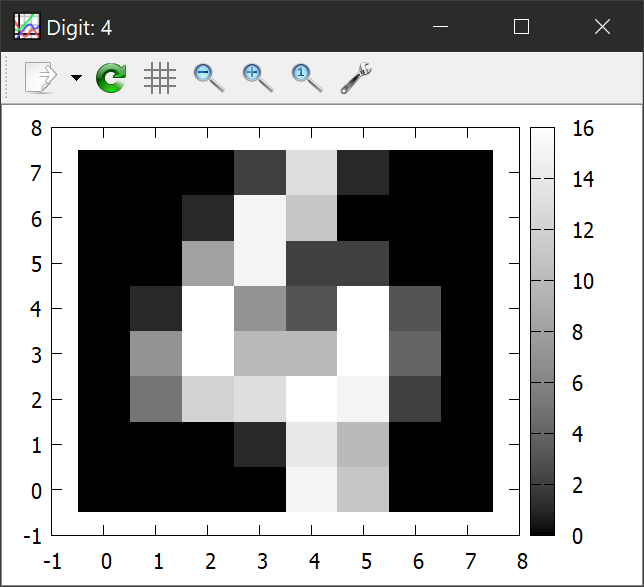
\includegraphics[width=5cm]{optical_digit/four_optical_digit.png}
            \caption{Conjunto de Datos Optical Digit}
            \label{fig:optical_digit}
        \end{figure}

        Este conjunto de datos se utiliza en diferentes áreas de la inteligencia artificial, tales como:
        
        \begin{enumerate}
            \item Clasificación de digitos.
            \item Reconocimiento de patrones.
            \item Comparación de modelos. 
            \item Aprendizaje supervisado.
        \end{enumerate}
        Al usar este tipo de conjunto de datos se obtienem algunas ventajas que por su simplicidad y tamaño permite que los test sean más rápidas que con otros.
    \subsection{Redes Neuronales Artificiales}

        Las redes neuronales artificiales (RNA) son modelos computacionales dentro de la Inteligencia Artificial que contienen unidades de procesamiento simples llamadas neuronas. Estas se inspiran en el cerebro humano, basándose en la conectividad entre neuronas y el aprendizaje que pueden tener. Un perceptrón o neurona (artificial) solo resuelve problemas lineales y tiene la siguiente forma:

        \begin{figure}[H]
            \centering
            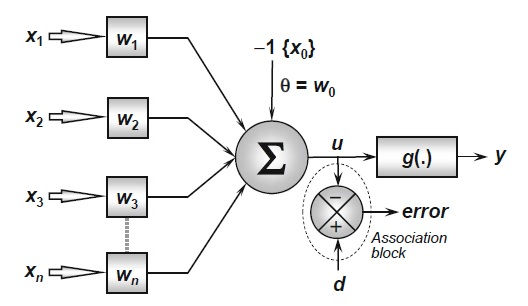
\includegraphics[width=\columnwidth]{neural_networks/multilayer_perceptron/ANN.jpg}
            \caption{Red Neuronal Artificial Básica}
            \label{fig:nerural_network}
        \end{figure}

        Donde $\Sigma$ es la representación matemática de la neurona. $x_1$, $x_2$, \dots ,$x_n$ son las variables de entrada a la red, y $w_1$, $w_2$, \dots ,$w_n$ son los pesos con los cuales se ponderan las entradas, es decir, se multiplican cuando la información entra en la neurona. Posteriormente, se suman todos esos valores: $w_1 x_1 + w_2 x_2 + w_3 x_3$. 

        Al revisar la fórmula anterioir, se puede observar que se parece a la operación de una regresión, la cual es: $y = w_0 + w_i x_i$. De esta manera, internamente la neurona realiza una regresión lineal. El parámetro que permite a la neurona trazar una recta cruzando el eje $y$ en el plano cartesiano (eje de las ordenadas) es conocido como sesgo (del inglés $bias$). Este valor se agrega a la conexión y usualmente se le asigna un valor de 1.

        Agregando este nuevo valor a la fórmula, queda de la siguiente manera: $y = \Sigma w_i x_i + w_0 b$, donde $b$ es el sesgo. 

        Sin embargo, se debe de tener presente que al usar una sola neurona, la única problemática que se puede resolver, son los problemas lineales, un ejemplo de esto es la resolución de problemas de puertas lógicas de tipo AND u OR, las cuales se presentan en la Figura \ref{fig:logic_gates}, si se necesita la resolución de problemas no lineales o también conocidos como puerta lógica de tipo XOR, Figura  \ref{fig:xor_logic_gate} no podrá, esto sucede ya que al ser un problema de tipo lienal no puede separar de manera correcta los datos que se le asigna, en cambio una resolución de problemas no lineales como lo es la puerta XOR permite realizar una correcta agrupación de clases (0 y 1), para poder realizarlo se debe de implementar las redes neuronales de multicapa, mejor conocidas como \textit{Perceptron Multicapa} las cuales permiten combinar n numero de capas neuronales. 

        \begin{figure}[H]
            \begin{subfigure}[H]{0.49\textwidth}
                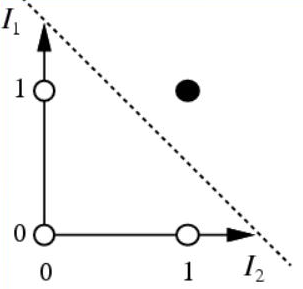
\includegraphics[width=\textwidth, height=\textwidth]{logic_gates/and.png}
                \caption{Puerta Lógica AND}
                \label{fig:and_logic_gate}
            \end{subfigure}
            \hfill
            \begin{subfigure}[H]{0.49\textwidth}
                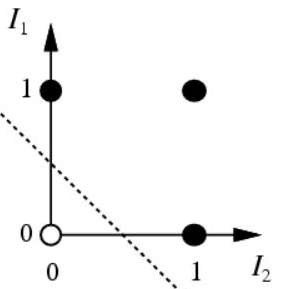
\includegraphics[width=\textwidth, height=\textwidth]{logic_gates/or.png}
                \caption{Puerta Lógica OR}
                \label{fig:or_logic_gate}
            \end{subfigure}
            \caption{Puertas Lógicas}
            \label{fig:logic_gates}
        \end{figure}

        \begin{figure}[H]
            \centering
            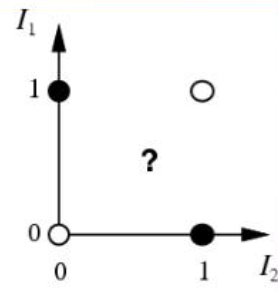
\includegraphics[width=5cm]{logic_gates/xor.png}
            \caption{Puerta Lógica XOR}
            \label{fig:xor_logic_gate}
        \end{figure}

        Además del uso de 2 o más capas dentro de la neurona, es indispensable el uso de una función de activación (Sección \ref{sec:activation}) que permite pasar la información de una neurona a otra dentro de un rango específico, lo cual se describirá en la siguiente sección.

        \subsubsection{Función de Activación} \label{sec:activation}

        Este método se utiliza cuando el modelo de RNA contiene dos o más neuronas, además proporciona al modelo una salida no lineal. Para este tipo de problemáticas donde tienen 3 entradas, se utiliza la siguiente fórmula: $f(w_1x_1 + w_2x_2 + w_3x_3 + b_0)$. Sin mencionar que las funciones de transferencia ayudan en cuestiones probabilísticas, ya que se representan en un rango de 0 a 1 \cite{renganathan2019}.

        Al hablar de funciones de activación, se deben comentar las más comunes:
        
        \begin{itemize}
            \item \textbf{Función Escalonada:} \\
                Esta función se utiliza para problemas de clasificación, ya que su salida es binaria, es decir, 0 o 1.
                \begin{figure}[H]
                    \centering
                    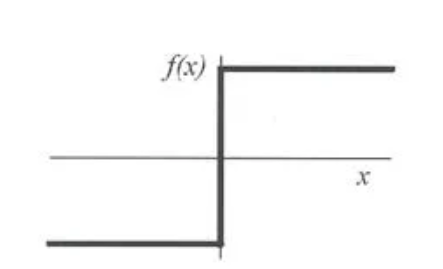
\includegraphics[width=5cm]{activation_functions/staggered.png}
                    \caption{Función Escalonada}
                    \label{fig:step_function}
                \end{figure}

                Dicha función está representada por:

                \[
                f(x) = \left\{ \begin{array}{lr} 
                0 & : x < 0 \\
                1 & : x \ge 0 
                \end{array} \right.
                \]
            
            \item \textbf{Función Sigmoide:} \\
                Esta función es una de las más comunes, ya que su salida es un rango de 0 a 1, lo que permite interpretarla como una probabilidad.
                \begin{figure}[H]
                    \centering
                    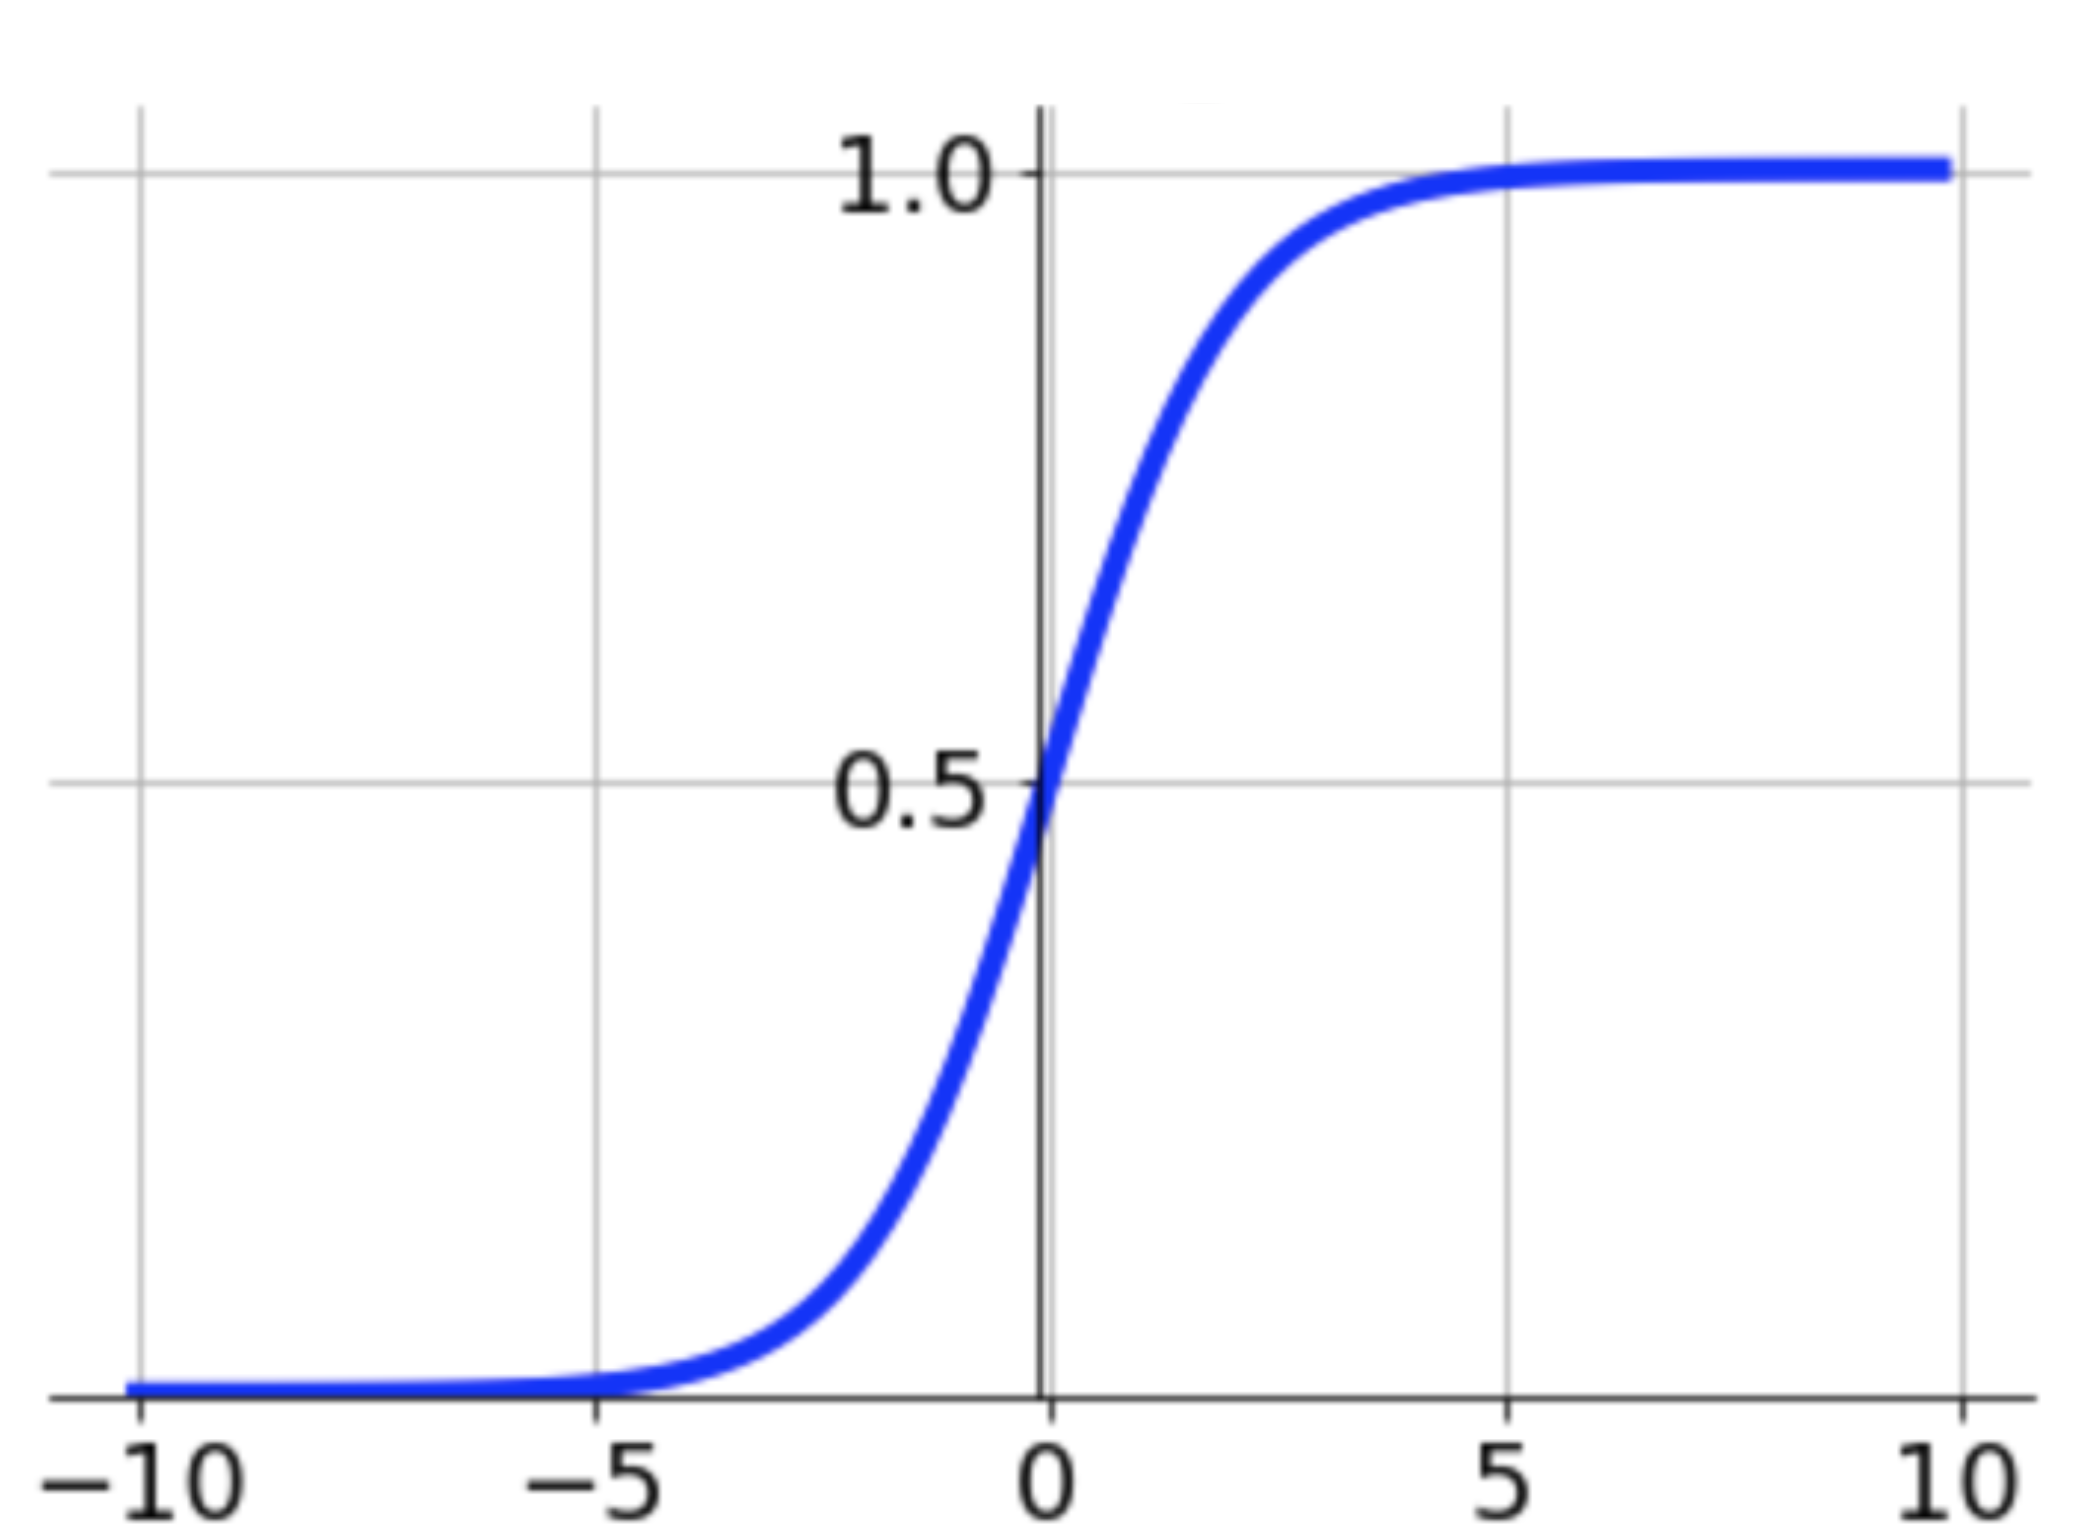
\includegraphics[width=5cm]{activation_functions/sigmoid.png}
                    \caption{Función Sigmoide}
                    \label{fig:sigmoid_function}
                \end{figure}

                Está representada por la siguiente fórmula:

                \[
                f(x) = \sigma(x) =  \frac{1}{1 + e^{-x}}
                \]

                Sin mencionar que este tipo de funciones es ajustable, lo cual es una característica importante del algoritmo de retropropagación (Sección: \ref{sec:backpropagation}).
            
            \item \textbf{Función de Unidad Rectificada Lineal (ReLU):} \\
                Esta función es la más utilizadas en RNAs ya que supera los problemas de desvanecimeinto del gradiente, además de ser más rápida en el entrenamiento. \\
                Es una función lineal que, cuando es positiva, toma el valor de la entrada, y cuando es negativa, toma el valor de 0.

                \begin{figure}[H]
                    \centering
                    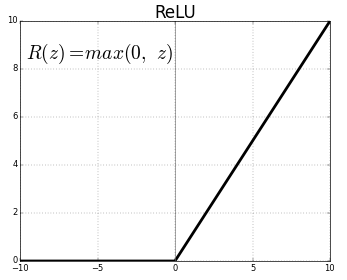
\includegraphics[width=6cm]{activation_functions/relu.png}
                    \caption{Función ReLU}
                    \label{fig:relu_function}
                \end{figure}

                Está representada por la siguiente fórmula:

                \[
                f(x) = \left\{ \begin{array}{lr} 
                0 & : x < 0 \\
                x & : x \ge 0 
                \end{array} \right.
                \]
            
            \item \textbf{Función Softmax:} \\
                Esta función se utiliza en la capa de salida de la red neuronal, ya que transforma las salidas en una representación probabilística, de tal manera que la suma de todas las probabilidades sea 1.
                \begin{figure}[H]
                    \centering
                    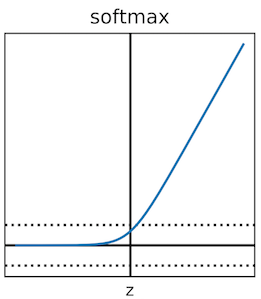
\includegraphics[width=6cm]{activation_functions/softmax.png}
                    \caption{Función Softmax}
                    \label{fig:softmax_function}
                \end{figure}

                Su representación matemática es:

                \[
                f(z)_j = \frac{e^{z_j}}{\sum_{K=1}^{K} e^{z_k}}
                \]
            
            \item \textbf{Función Tangente Hiperbólica:} \\
                Esta función es similar a la función sigmoide, pero su rango es de -1 a 1. También sufre de problemas de desvanecimiento del gradiente, lo que puede dificultar el entrenamiento de redes neuronales profundas.

                \begin{figure}[H]
                    \centering
                    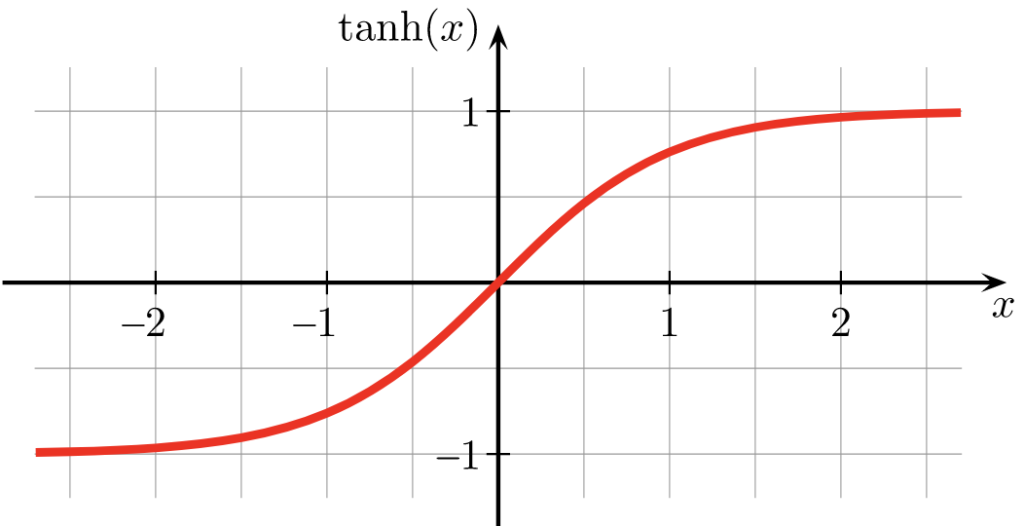
\includegraphics[width=6cm]{activation_functions/tanh.png}
                    \caption{Función Tangente Hiperbólica}
                    \label{fig:tanh_function}
                \end{figure}

                Su representación matemática es:

                \[
                f(x) = \tanh(x) = \frac{e^x - e^{-x}}{e^x + e^{-x}}
                \]
        
        \end{itemize}
        
        Las redes neuronales presentan diversas utilidades que ayudan a resolver problemas como no linealidad, mapeo entrada-salida, aprendizaje robusto a errores en los datos de entrenamiento, entre otros. Existen varios tipos de redes neuronales, como las redes neuronales de perceptrón multicapa y redes neuronales convolucionales, que se describirán brevemente más adelante.

    \subsection{Redes Neuronales de Perceptrón Multicapa}

        Las Redes Neuronales de Perceptrón Multicapa (MLP) pueden dividirse en dos capas (entrada y salida), pero también pueden tener tres o más capas (entrada, una o más capas ocultas y salida). En las capas ocultas, se pueden tener más de una fila de neuronas, que son las encargadas de realizar las operaciones para eliminar la linealidad de los datos. Como se comentó anteriormente en la sección \ref{sec:activation}, la linealidad de los datos se elimina con las funciones de activación, que modifican los parámetros de la red, permitiendo la elaboración de un plano tridimensional con el cual se puede encontrar la solución al problema planteado.

        Además, como se explicó anteriormente, no es recomendable trabajar con una sola neurona debido a los problemas al resolver tareas como XOR, donde se requieren dos líneas rectas para clasificar el problema correctamente.

        Como se puede observar en la Figura \ref{fig:multilayer_perceptron}, para este caso se cuenta con una MLP que consta de 4 capas: una de entrada, dos ocultas y una de salida. En las capas ocultas y de salida se lleva a cabo el procesamiento de las funciones de activación, mientras que en la capa de entrada no se aplica ninguna función de transferencia, ya que simplemente representa las entradas al modelo.

        \begin{figure}[H]
            \centering
            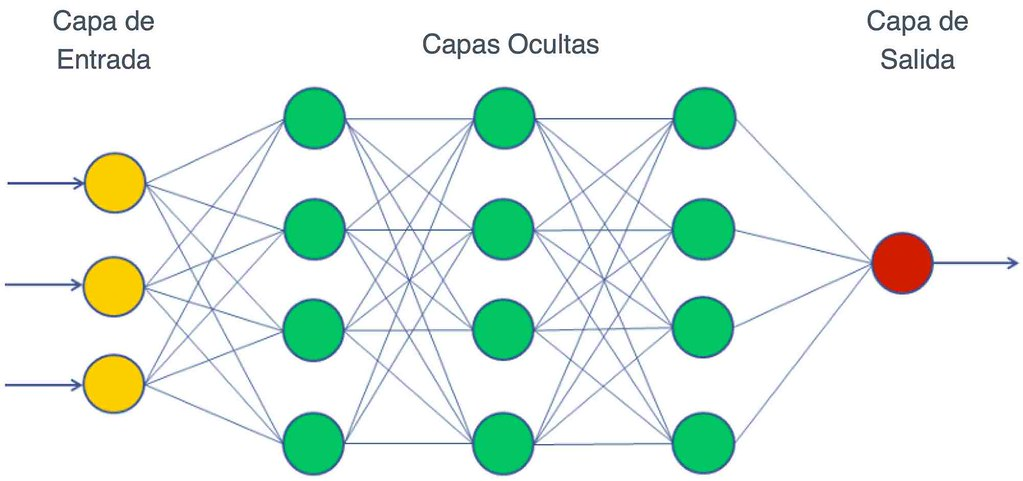
\includegraphics[width=\columnwidth]{neural_networks/multilayer_perceptron/multipercep.jpg}
            \caption{Red Neuronal Multicapa}
            \label{fig:multilayer_perceptron}
        \end{figure}

    \subsection{Algoritmo de Retropropagación} \label{sec:backpropagation}

        El algoritmo de retropropagación es un algoritmo de aprendizaje que permite que una red neuronal autoajuste todos sus parámetros para aprender una representación interna de la información que está procesando. Llegó para resolver la limitante del perceptrón, que solo resuelve problemas lineales, y se extiende a redes más complejas, es decir, a problemas no lineales.

        Mediante este algoritmo se obtienen las derivadas parciales del gradiente y los pesos, los cuales se utilizan para optimizar la red neuronal. También se deben calcular las derivadas del sesgo, que indican en qué capa se encuentra el error. El uso de estas derivadas parciales permite encontrar el error, y lo que realiza el algoritmo es retroceder hasta la neurona donde se encuentra el error, regresando desde la capa de salida hasta la capa de entrada.

        Para poder realizar todo este proceso de retropropagación, es necesario contar con una función de activación diferenciable.

    \subsection{Redes Neuronales Convolucionales}

        Las Redes Neuronales Convolucionales (CNN, por sus siglas en inglés) son redes profundas con una estructura especial. Están conformadas por tres tipos de capas: convolucionales, de agrupación y completamente conectadas.

        En las capas convolucionales, el filtro detecta características específicas dentro de la imagen de entrada, como bordes, colores, o texturas, y genera un mapa de características. En las capas de agrupación, se reduce la resolución espacial de la imagen, lo que permite reducir la cantidad de parámetros y el costo computacional. Finalmente, las capas completamente conectadas están encargadas de realizar la clasificación.

        Las CNN son muy útiles para el reconocimiento de imágenes, y se han utilizado en una amplia variedad de aplicaciones, desde la visión por computadora hasta la medicina y el reconocimiento de voz.


    \subsection{Aprendizaje Incremental}

        Con el paso del tiempo, la tecnología ha evolucionado, lo que ha llevado a un aumento en la cantidad de datos disponibles. El aprendizaje automático ha experimentado avances significativos, y los datos se generan y procesan con mayor frecuencia.

        Se puede definir una tarea de aprendizaje como incremental si los ejemplos de entrenamiento utilizados para resolverla se presentan de manera secuencial, generalmente uno a la vez. Si los resultados no son urgentes, este tipo de tareas puede ser resuelto mediante algoritmos de aprendizaje no incremental \cite{GiraudCarrier2000}. Un área donde el aprendizaje incremental es especialmente útil es en la \textit{robótica}, ya que estos sistemas requieren entrenamiento constante \cite{GiraudCarrier2000}.

        Este enfoque de aprendizaje fue inspirado por la forma en que los seres humanos aprenden y es más rápido, lo que llevó a su adopción en el campo del aprendizaje automático.

        Con el tiempo, el aprendizaje incremental se ha convertido en un paradigma del aprendizaje automático, donde el sistema toma nuevos ejemplos y los agrega a los ya aprendidos. A medida que el sistema aprende, los ejemplos previos pueden ser reemplazados por los nuevos \cite{liu2015}.

        \subsubsection{Algoritmos de Aprendizaje Incremental}

            Un algoritmo de aprendizaje incremental se define por los siguientes criterios:
            \begin{enumerate}
                \item Ser capaz de aprender y actualizarse con cada nuevo dato, etiquetado o no etiquetado.
                \item Conservar el conocimiento adquirido previamente.
                \item No requerir acceso a los datos originales.
                \item Ser capaz de generar nuevas clases o clusters cuando sea necesario, así como dividir o fusionar clusters según lo requiera el entorno.
                \item Tener una naturaleza dinámica, adaptándose a un entorno cambiante \cite{Deshmukh2013}.
            \end{enumerate}

            \begin{figure}[H]
                \centering
                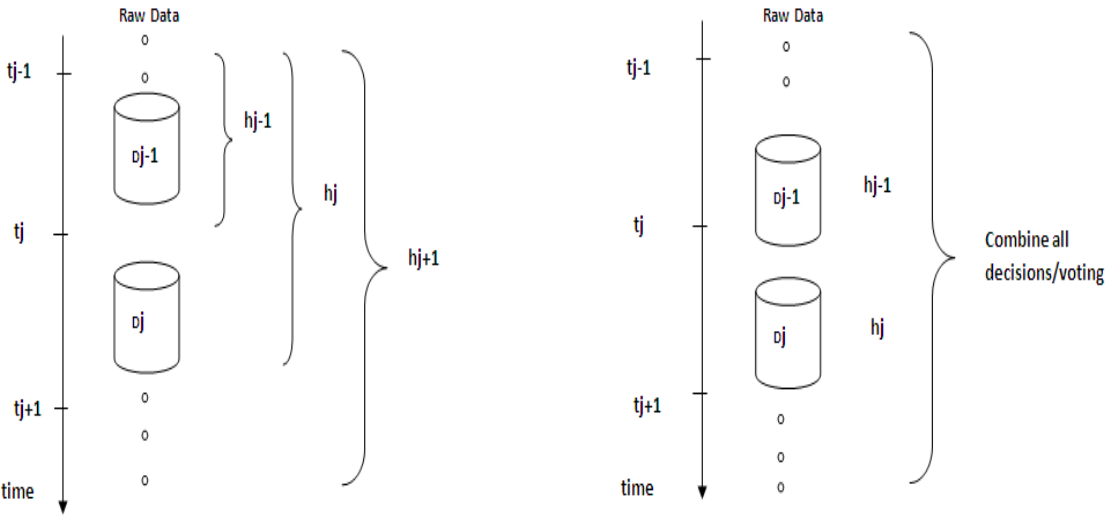
\includegraphics[width=\columnwidth]{incremental_learning/incremental_learning_methods.png}
                \caption{Dos enfoques tradicionales del aprendizaje incremental.}
                \label{fig:incremental_learning_algorithm}
            \end{figure}

            Como se observa en la Figura 11, el primer enfoque consiste en la acumulación de datos, donde, al recibir una nueva porción de datos \(D_j\), se descarta la hipótesis \(h_{j-1}\) y se genera una nueva hipótesis \(h_j\) basada en todos los datos disponibles hasta ese momento. En el segundo enfoque, al recibir una nueva porción de datos \(D_j\), se desarrolla una única hipótesis nueva o un conjunto de hipótesis nuevas basadas en los nuevos datos. Finalmente, se puede usar un mecanismo de votación para combinar todas las decisiones de las diferentes hipótesis y obtener la predicción final.

            El aprendizaje incremental tiene la ventaja de no requerir almacenamiento de los datos previos, ya que el conocimiento se guarda en las hipótesis generadas durante el proceso de aprendizaje.

            \begin{quote}
                \textit{``Un algoritmo de aprendizaje es incremental si, para cualquier muestra de entrenamiento dada:
                \begin{equation*}
                    e_1, e_2, ..., e_s
                \end{equation*}
                produce una secuencia de hipótesis
                \begin{equation*}
                    h_0, h_1, ..., h_n
                \end{equation*}
                tal que \(h_{i+1}\) depende solo de \(h_i\) y de la muestra actual \(e\)\cite{GiraudCarrier2000}.''}
            \end{quote}

            Como se observa, estos algoritmos permiten que la inteligencia artificial realice tareas de predicción de manera más eficiente.

            Un ejemplo de esta metodología es el proyecto \textit{COBWEB}, que categoriza el número de clusters y la pertenencia de dichos clusters utilizando una métrica probabilística global. Este proceso implica agregar nuevas categorías, actualizando las probabilidades con los nuevos datos recolectados \cite{fisher1987}.
    
    \subsection{Estado del Arte}
